\section{Results}
In this section, the main results of the analysis will be shown. Given the twofold goal of this work, two sections will be needed. One for the performance of the strategy and one analyzing the PnL drivers of said performance. 

\subsection{Strategy}
In this section, the performance of the strategy will be shown. First, it will be presented in comparison to the overall market, then as a comparison to the calculated benchmark and finally disaggregating the long and short legs of the strategy. 

\subsubsection{Overall Performance}
\label{sec:overall-performance}
In order to showcase the performance of the newly implemented strategy, several visual representations and usual metrics for measuring performance and risk will be shown in comparison with the S\&P500 as a very basic reference point. 

\begin{figure}[ht]
    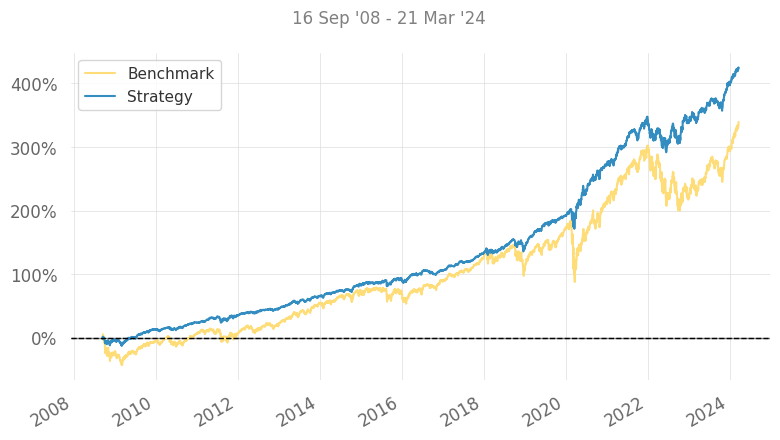
\includegraphics[width=\linewidth]{assets/strat-vs-sp500.png}
    \caption{Cumulative returns of the strategy compared with the S\&P500}
    \label{fig:strat-vs-sp500}
\end{figure}

The most basic way in which one can start to see the performance of the trading strategy is looking at how the cumulative returns evolve over time compared with the S\&P500. In \autoref{fig:strat-vs-sp500} it can be seen how the overall cumulative returns are higher, and seemingly less volatile. 
In order to understand whether the volatility truly is lower, a useful visualization is the volatility-matched returns of the strategy.

\begin{figure}[ht]
    \captionsetup{justification=centering}
    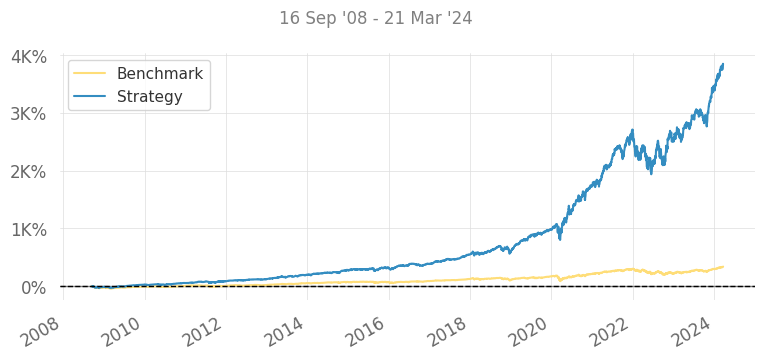
\includegraphics[width=\linewidth]{assets/strat-vs-sp500-vol-matched.png}
    \caption{Cumulative returns of the volatility matched strategy compared with the S\&P500}
    \label{fig:strat-vs-sp500-vol-matched}
\end{figure}
These are the returns that would be obtained investing in the strategy if the position were leveraged enough to match the volatility of the S\&P500. That is, if the investor were to borrow enough money and put it in the strategy so that the volatility of said setup is the same volatility as the benchmark. The returns are thus:
\begin{equation}
    r_{vm}=\frac{\sigma_b}{\sigma_s}r_s
\end{equation}
where $r_{vm}$ are the volatility matched returns, $\sigma_b$ is the benchmark's volatility, $\sigma_s$ is the strategy's volatility and $r_s$ is the strategy's returns. 
If a given investor is comfortable enough with the level of risk given by a basic market investment, these are the equivalent results that could be obtained with the given strategy.

Appart from visualizing the cumulative performance, it will also be helpful to showcase some numerical results. 

\begin{table}[ht]
    \centering
    \begin{tabular}{rll}
        \toprule
        Metric & \multicolumn{2}{c}{Value} \\ 
        \cmidrule(lr){2-3}
            & Strategy & S\&P500 \\
        \midrule
        CAGR & 7.65\% & 6.81\% \\
        Annualized Volatility & 8.79\% & 20.45\% \\
        Skew & 0.14 & -0.29 \\
        Kurtosis & 7.9 & 12.65 \\
        \bottomrule
    \end{tabular}
    \caption{Main moments of the strategy's return distribution}
    \label{table:main-moments-strat-vs-sp500}
\end{table}

As a sidenote, it can be seen how the CAGR for the S\&P500 is much lower than the mean annual returns that have been recorded during this period. That is because the CAGR takes into account how the price movements compound over time, and thus volatility, skewness and kurtosis effects are also present. The mean compounded returns are thus not $r_c=\mu$, but 
\begin{equation}
    r_c=\mu-\frac{1}{2}\sigma^2+\frac{1}{3}S\sigma^3-\frac{1}{4}K\sigma^4  + \mathcal{O}\left(\sigma^5\right)
\end{equation}
where $\mu$ are the mean annual returns, $\sigma$ is the annualized standard deviation of the returns, $S$ is the skewness and $K$ is the kurtosis of the return distribution. This is thus a more representative figure of the expected long term returns than if mean annual returns were showcased here.

In \autoref{table:main-moments-strat-vs-sp500} four metrics referring to the four first moments of the return distributions can be seen. 
It confirms numerically what was already intuited by watching the cumulative distribution of \autoref{fig:strat-vs-sp500}, returns are higher on average and risk -- as measured by the volatility -- is lower. However, by looking at the next two moments more interesting information is uncovered. While stock returns are well known to generally exhibit a negative skew as shown in \cite{peiro_1999} and confirmed here with the S\&P500 returns, the strategy manages to obtain positive skew returns. Similarly for kurtosis, even though the strategy's value still lies above the normal distribution's 3, it is considerably lower than the market's kurtosis.

This can be visualized very nicely in \autoref{fig:strat-vs-sp500-ret-dist}, where the monthly return distribution for both sets of returns are shown. 

\begin{figure}[ht]
    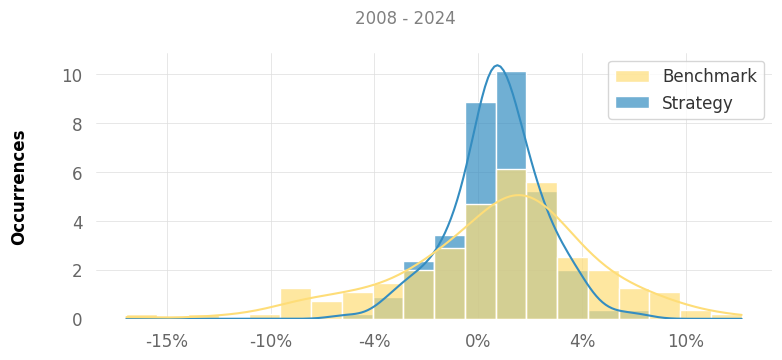
\includegraphics[width=\linewidth]{assets/strat-vs-sp500-ret-dist.png}
    \caption{Monthly returns distribution of the strategy compared with the S\&P500}
    \label{fig:strat-vs-sp500-ret-dist}
\end{figure}

Apart from the already presented metrics, which are seen clearly in the distribution plot, it can be seen how it could seem like the mean of the distribution for the S\&P500 is higher than that of the strategy. However, the only thing that is clearly higher is the mode, and the more extreme negative movements experienced by the benchmark really weigh down on the long run average compounded returns. 

Some other risk-adjusted measures for the strategy are 
\begin{table}[ht]
    \centering
    \begin{tabular}{rll}
        \toprule
        Metric & \multicolumn{2}{c}{Value} \\ 
        \cmidrule(lr){2-3}
            & Strategy & S\&P500 \\
        \midrule
        Sharpe ratio & 1.16 & 0.51 \\
        Sortino ratio & 1.69 & 0.73 \\
        Calmar ratio & 0.54 & 0.15 \\
        Max Drawdown & -14.15\% & -46.1\% \\
        Longest Drawdown & 335 & 821 \\
        Alpha & 0.12 & - \\
        Beta & -0.06 & - \\
        Correlation & -13.88\% & - \\
        Treynor ratio & -7103.63\% & - \\
        \bottomrule
    \end{tabular}
    \caption{Risk and risk-adjusted return metrics for the strategy}
    \label{table:risk-adjusted-strat-vs-sp500}
\end{table}

In \autoref{table:risk-adjusted-strat-vs-sp500} the intuition gained with the previous metrics is solidified. Through the main risk-adjusted return metrics it can be seen how the strategy's performance is clearly superior to that of the S\&P500. Regarding other purely risk measures like those relative to drawdowns, it can also be seen how the periods of losses with the strategy are less acute and shorter. Finally, it can also be seen how the strategy's performance is completely market neutral if not slightly opposite to the market, with a slightly negative beta and correlation. This means that the strategy can be effectively used as a hedge to a market investment, partially compensating in moments of low or negative market returns. The superior performance together with the hedging and diversification potential it brings provides for a very significant alpha. 

For a more in depth explanation of these metrics, how they are calculated and their general interpretation and significance refer to \autoref{sec:performance-metrics-explained} \nameref{sec:performance-metrics-explained}.

When taking a dynamic view of these figures, it can be seen how temporally robust the findings are.

\begin{figure}[ht]
    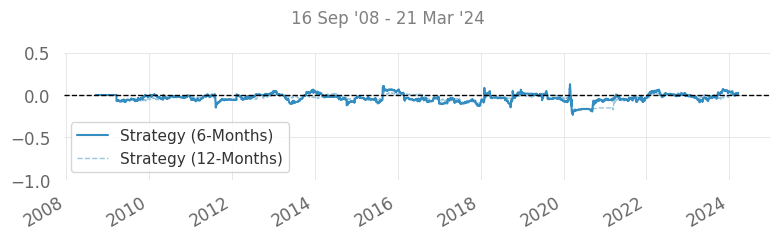
\includegraphics[width=\linewidth]{assets/strat-vs-sp500-rolling-beta.png}
    \caption{6 and 12 month rolling beta of the strategy's returns with respect to the S\&P500}
    \label{fig:strat-vs-sp500-rolling-beta}
\end{figure}

In \autoref{fig:strat-vs-sp500-rolling-beta} the rolling beta can be seen. That is, at each point in time the beta obtained with the previous 6 or 12 month window. Observing this figure it can be seen how the beta of the strategy stays consistently very close to zero and generally on the negative side, with very few ocurrences of the beta becoming positive. It is specially significant how in the moments of biggest crisis, i.e. the 2020 Covid-19 market crash, the beta becomes even more significantly negative showcasing the resilience of the strategy to market crashes. This is conforms perfectly with the results obtained by \cite{ioannis_2023}. This behaviour is specially relevant given the findings by \cite{sandoval_franca_2012} showing that during market crashes most assets become a lot more strongly correlated, making it even more difficult for investors to diversify their investments in these times. 

% Finally, some other more practical metrics that could be useful from the trading perspective
% \begin{table}[ht]
%     \centering
%     \begin{tabular}{rll}
%         \toprule
%         Metric & \multicolumn{2}{c}{Value} \\ 
%         \cmidrule(lr){2-3}
%             & Strategy & S\&P500 \\
%         \midrule
%         Sharpe ratio & 1.16 & 0.51 \\
%         Sortino ratio & 1.69 & 0.73 \\
%         Omega ratio & 0.14 & -0.29 \\
%         Max Drawdown & -14.15\% & -46.1\% \\
%         Longest Drawdown & 335 & 821 \\
%         Alpha & 0.12 & -- \\
%         Beta & -0.06 & -- \\
%         Correlation & -13.88\% & -- \\
%         Treynor ratio & -7103.63\% & -- \\
%         \bottomrule
%     \end{tabular}
%     \caption{Risk and risk-adjusted return metrics for the strategy}
%     \label{table:risk-adjusted-strat-vs-sp500}
% \end{table}

A final aspect of the performance of the strategy which has not been discussed until this point is the number of trades or assets it effectively enters positions in. This can be seen in \autoref{fig:strat-open-pairs}.

\begin{figure}[ht]
    \captionsetup{justification=centering}
    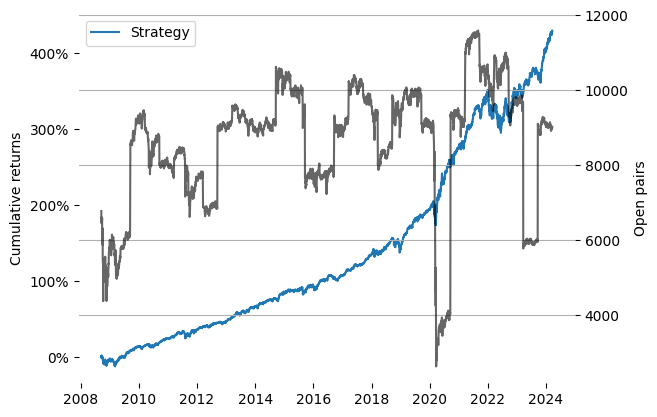
\includegraphics[width=\linewidth]{assets/strat-open-pairs.png}
    \caption{Pairs with open positions taken by the strategy together with the cumulative returns}
    \label{fig:strat-open-pairs}
\end{figure}

In \autoref{fig:strat-open-pairs} it can be seen that at any given point there are between $\sim$12.000 and $\sim$3.000 pairs being traded, with the average being around $\sim$9.000. For a position to be open in a given pair, that pair needs to have been found to be cointegrated in the previous time period, and in the current day the trading trigger needs to have been activated. In 500 stocks, the total possible number of pairs is of 124.750. However, not all 500 stocks have been members of the index for the whole time period, so only 398 stocks are effectively used, which gives a total of 79.003 potential pairs. This means, that on average the strategy is trading $\sim$11\% of all possible pairs. 

It is also relevant how there doesn't seem to be any clear relationship between the number of pairs being traded and the distribution of returns, with returns behaving similarly in periods of high volume of open positions and in periods of low volume of open positions. 

\subsubsection{Comparison with Johansen Portfolio}
After having seen in general terms what the performance of the strategy looks like, it is pertinent now to compare it with a more similar strategy, that of the Johansen cointegration portfolio. This is another pairs-trading cointegration based strategy, and thus it is expected to be a lot more similar than to the S\&P500. The general comparison of the cumulative returns of both is the following:

\begin{figure}[ht]
    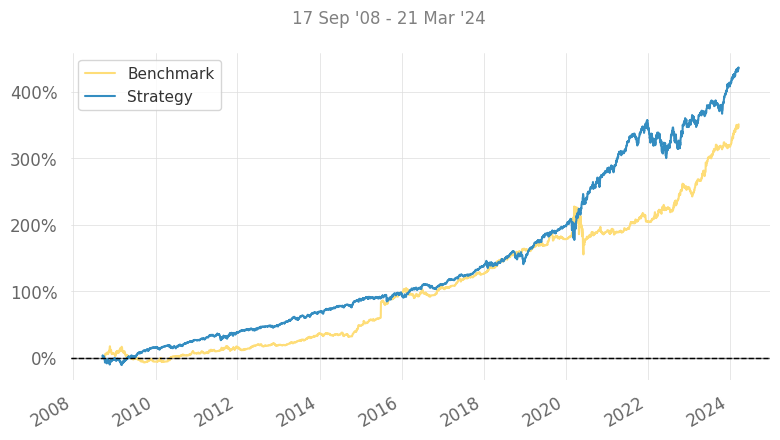
\includegraphics[width=\linewidth]{assets/strat-vs-johansen.png}
    \caption{Cumulative returns of the strategy compared with the S\&P500}
    \label{fig:strat-vs-johansen}
\end{figure}

From a first glance it can be seen how this is a much more even comparison than with the S\&P500. The performance of the Johansen portfolio exhibits higher overall cumulative returns and apparently lower volatility throughout the period. However, the overall returns of the selected strategy still lie above those of the Johansen portfolio. As for the volatility, it is hard to judge simply graphically, and thus the precise numbers are shown in \autoref{table:main-moments-strat-vs-johansen}

\begin{table}[ht]
    \centering
    \begin{tabular}{rll}
        \toprule
        Metric & \multicolumn{2}{c}{Value} \\ 
        \cmidrule(lr){2-3}
            & Strategy & Johansen \\
        \midrule
        CAGR & 7.65\% & 6.93\% \\
        Annualized Volatility & 8.79\% & 8.84\% \\
        Skew & 0.14 & 3.03 \\
        Kurtosis & 7.9 & 92.03 \\
        \bottomrule
    \end{tabular}
    \caption{Main moments of the strategy's return distribution}
    \label{table:main-moments-strat-vs-johansen}
\end{table}

It can be seen how the annual returns are ever so slightly superior for the strategy compared to the Johansen portfolio and the annualized volatility is actually lower, although marginally. However, the comparison for the skew and kurtosis should be made more carefully. If the cumulative returns graph for the Johansen portfolio in \autoref{fig:strat-vs-johansen} is inspected carefully, it becomes apparent how in 2020 -- during the midst of the Covid-19 market crash -- there is a very abrupt movement in the cumulative reutrns graph. Due to the positions taken by the Johansen strategy, there is a great profit and then loss, which accentuates the weight of the extremes and biases the kurtosis metric. The similarity between both distributions can be better seen graphically in \autoref{fig:strat-vs-johansen-ret-dist}.

\begin{figure}[ht]
    \captionsetup{justification=centering}
    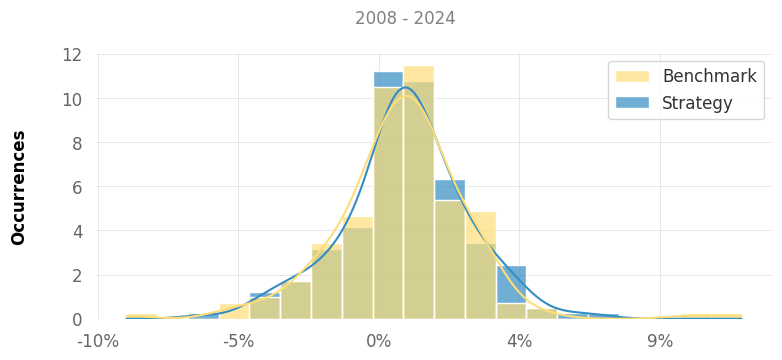
\includegraphics[width=\linewidth]{assets/strat-vs-johansen-ret-dist.png}
    \caption{Monthly returns distribution of the strategy compared with the Johansen portfolio}
    \label{fig:strat-vs-johansen-ret-dist}
\end{figure}

In \autoref{fig:strat-vs-johansen-ret-dist} it is made apparent how both distributions are much more similar than what may appear through the skew and kurtosis numbers. It can be seen in fact how the proposed pairs-trading strategy has a return distribution practically equal to its pairs-trading vanilla equivalent. It is due to high frequency of returns at around the $\sim$90\% percentile that the proposed strategy's superior performance is materialized.    

If a more practical comparison wants to be made, it could be useful to again look at the same metrics already shown in \autoref{table:risk-adjusted-strat-vs-sp500} but comparing the strategy to its new benchmark. 

\begin{table}[ht]
    \centering
    \begin{tabular}{rll}
        \toprule
        Metric & \multicolumn{2}{c}{Value} \\ 
        \cmidrule(lr){2-3}
            & Strategy & S\&P500 \\
        \midrule
        Sharpe ratio & 1.16 & 1.03 \\
        Sortino ratio & 1.69 & 1.59 \\
        Calmar ratio & 0.54 & 0.31 \\
        Max Drawdown & -14.15\% & -22.0\% \\
        Longest Drawdown & 335 & 1032 \\
        Alpha & 0.11 & -- \\
        Beta & -0.0 & -- \\
        Correlation & -0.18\% & -- \\
        \bottomrule
    \end{tabular}
    \caption{Risk and risk-adjusted return metrics for the strategy}
    \label{table:risk-adjusted-strat-vs-johansen}
\end{table}

A clear dominance by the strategy, although by margins much smaller than in the previous comparison, can be seen across all metrics. This dominance is most apparent in the drawdown statistics, where the Johansen portfolio falls prey to a long period of bad performance after the 2020 crash. The alpha of the strategy with respect to the Johansen portfolio is also apparent. And very interestingly, although both strategies are sources of uncorrelated returns, following the same principle of cointegration leveraged through pairs-trading, the correlation between both strtegies is virtually non existant. Although operating under the same principles, it seems like both strategies are able to find different pairs and take different positions throughout the whole time period. Furthermore, the pair selection method introduced in \cite{ioannis_2023} and implemented here has some advantages apart from performance related ones like finding more pairs and better performing ones. It also can be performed on a greater universe of assets in a computationally more efficient and faster way than the Johansen pair selection method. 

\subsubsection{Disaggregated Performance}
In previous sections, the general performance of the strategy as a whole has been thoroughly analyzed, against the universe of assets and against a more comparable benchmark. However, this being a pairs-trading strategy offers a possible level of analysis that hasn't been much exploited until now in the literature. It is possible to disaggregate the performance of the strategy into the long and the short leg of the strategy -- that is, the performance of all operations where the strategy went long on a stock and those where it went short on a stock -- and analyze each sepparately, observing what features of the final strategy are brought by each half. 

\subsubsubsection{Long leg}
When first looking at the long leg of the strategy's cumulative returns compared to the strategy's cumulative returns, it may seem like just by keeping the long leg better performance can be achieved.

\begin{figure}[ht]
    \captionsetup{justification=centering}
    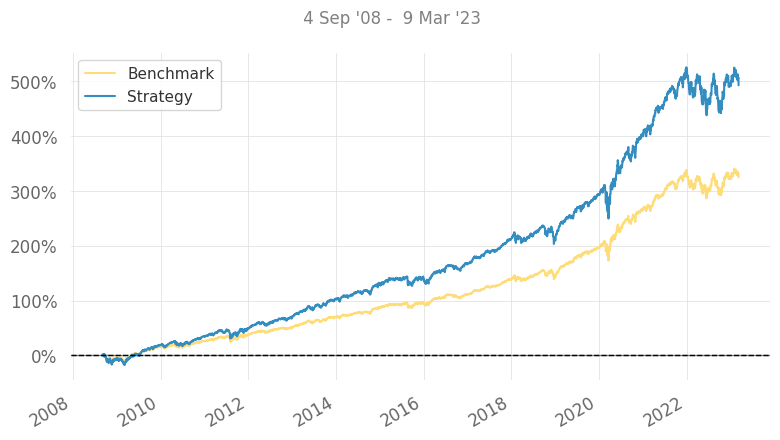
\includegraphics[width=\linewidth]{assets/long-vs-strat.png}
    \caption{Cumulative returns of the long leg of the strategy compared with the complete strategy}
    \label{fig:long-vs-strat}
\end{figure}

As it can be seen in \autoref{fig:long-vs-strat}, the overall returns of the long leg seem to be superior. However, upon closer inspection it is seen how this is only achieved through higher volatility. In fact, when matching the volatility of both these are the results:
\begin{figure}[ht]
    \captionsetup{justification=centering}
    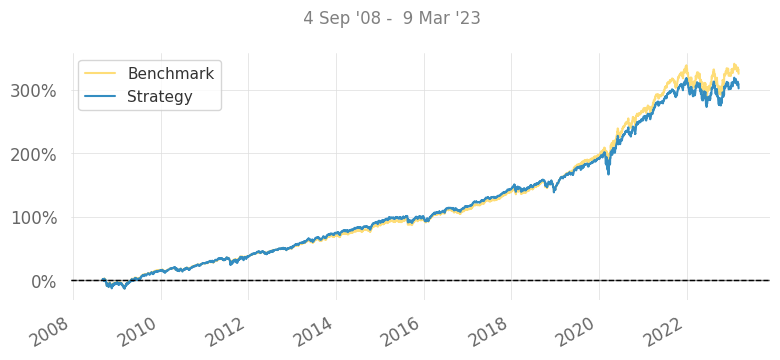
\includegraphics[width=\linewidth]{assets/long-vs-strat-vol-matched.png}
    \caption{Cumulative returns of the volatility matched long leg of the strategy compared with the strategy}
    \label{fig:long-vs-strat-vol-matched}
\end{figure}

A very interesting observation can be extracted from \autoref{fig:long-vs-strat-vol-matched}. At first, it may seem like the long leg of the strategy is just a leveraged position of the overall strategy. However, towards the end it becomes apparent how adding the short positions contributes to a very slight edge in volatility matched performance.

To see more precisely what this behaviour means in quantitative terms, the four first moments are presented in \autoref{table:main-moments-long-vs-strat}

\begin{table}[ht]
    \centering
    \begin{tabular}{rll}
        \toprule
        Metric & \multicolumn{2}{c}{Value} \\ 
        \cmidrule(lr){2-3}
            & Long leg & Strategy \\
        \midrule
        CAGR & 9.52\% & 7.65\% \\
        Annualized Volatility & 11.46\% & 8.79\% \\
        Skew & 0.04 & 0.14 \\
        Kurtosis & 6.01 & 7.9 \\
        \bottomrule
    \end{tabular}
    \caption{Main moments of the long leg of the strategy's return distribution}
    \label{table:main-moments-long-vs-strat}
\end{table}

As it could be inferred from previous observations in \autoref{fig:long-vs-strat} and \autoref{fig:long-vs-strat-vol-matched}, the mean returns and volatility of the long part of the strategy are higher than those of the strategy itself. However, looking at the third and fourth moments something more interesting comes to light. If the long portion of the strategy truly behaved like a leveraged position of the whole strategy, the skew and kurtosis would remain constant. However, the long leg exhibits a lower skew than the complete strategy, providing lower long term compound returns and more exposure to catastrophic tail negative return scenarios. Regarding the kurtosis of the distribution, it is also not the same. In this case, adding the negative positions increases this fourth moment, supposedly due to some extreme movements that are exhibited by the short leg of the strategy. This higher kurtosis, together with a positive skew, means that tail positive events are larger for the complete strategy and this facilitates having better performance with lower risk. All of this can be seen more clearly in \autoref{fig:long-vs-strat-ret-dist}.

\begin{figure}[ht]
    \captionsetup{justification=centering}
    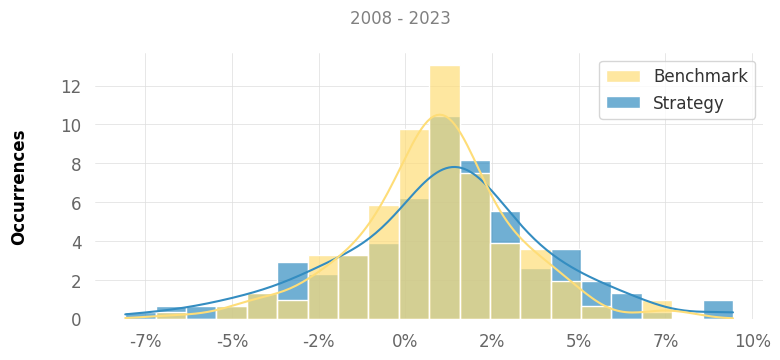
\includegraphics[width=\linewidth]{assets/long-vs-strat-ret-dist.png}
    \caption{Monthly returns distribution of the long leg of the strategy compared with the overall strategy}
    \label{fig:long-vs-strat-ret-dist}
\end{figure}

In order to understand on more practical terms what these differences in returns mean, the following metrics can be analyzed.

\begin{table}[ht]
    \centering
    \begin{tabular}{rll}
        \toprule
        Metric & \multicolumn{2}{c}{Value} \\ 
        \cmidrule(lr){2-3}
            & Long leg & Strategy \\
        \midrule
        Sharpe ratio & 1.12 & 1.16 \\
        Sortino ratio & 1.65 & 1.69 \\
        Calmar ratio & 0.51 & 0.54 \\
        Max Drawdown & -18.56\% & -14.15\% \\
        Longest Drawdown & 336 & 335 \\
        Alpha & -0.01 & -- \\
        Beta & 1.29 & -- \\
        Treynor ratio & 519.42\% & -- \\
        \bottomrule
    \end{tabular}
    \caption{Risk and risk-adjusted return metrics for the long leg of the strategy}
    \label{table:risk-adjusted-long-vs-strat}
\end{table}

By observing these metrics the similarity in perfromance between both sets of returns is again apparent. Most ratios, like the Sharpe ratio, Sortino ratio or Calmar ratio are slightly more favourable to the complete strategy, in accordance with the slightly superior volatility adjusted performance. Moreover, the leveraged looking behaviour is apparent in the beta above 1. However, as it can be seen in the rest of the ratios, this leveraged but slighly worse performance is reflected in the slightly negative alpha. 

\subsubsubsection{Short leg}

After having looked at the long leg, it is now time to look at how the performance of the short leg compares with the overall strategy. The best introduction is again the comparison of the short leg of the strategy's cumulative returns with the strategy's cumulative returns.

\begin{figure}[ht]
    \captionsetup{justification=centering}
    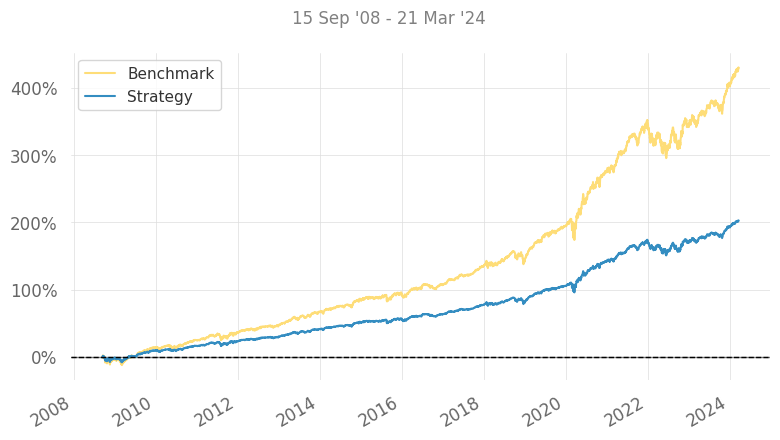
\includegraphics[width=\linewidth]{assets/short-vs-strat.png}
    \caption{Cumulative returns of the short leg of the strategy compared with the complete strategy}
    \label{fig:short-vs-strat}
\end{figure}

In this case, it can be seen how the situation seems to be the inverse one. The overall returns seem to be lower, albeit that also seems to imply a lower volatility. Referring to the volatility matched comparison is again a good reference point for checking whether these intuitions seem correct.
\begin{figure}[ht]
    \captionsetup{justification=centering}
    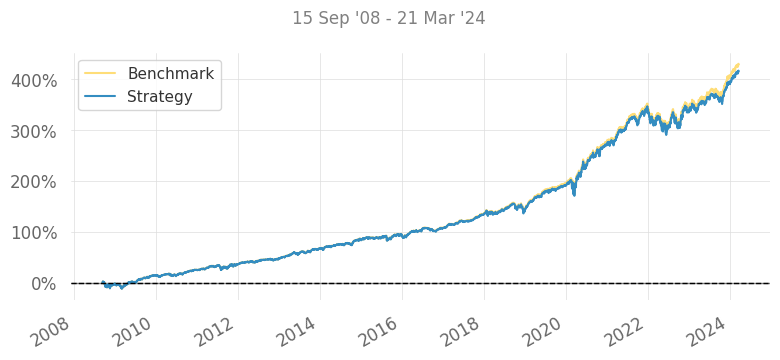
\includegraphics[width=\linewidth]{assets/short-vs-strat-vol-matched.png}
    \caption{Cumulative returns of the volatility matched short leg of the strategy compared with the strategy}
    \label{fig:short-vs-strat-vol-matched}
\end{figure}

Even though the performance seemed to be the opposite to that of the long leg -- lower performance through lower volatility -- in \autoref{fig:short-vs-strat-vol-matched} it can be seen that both are more similar than it would seem. The volatility matched performance is again very similar to that of the complete strategy, with a slight edge becoming again apparent towards the end of the period.

Referring again to the four first moments can be helpful in shedding some quantiative light.

\begin{table}[ht]
    \centering
    \begin{tabular}{rll}
        \toprule
        Metric & \multicolumn{2}{c}{Value} \\ 
        \cmidrule(lr){2-3}
            & Short leg & Strategy \\
        \midrule
        CAGR & 5.05\% & 7.65\% \\
        Annualized Volatility & 5.86\% & 8.79\% \\
        Skew & 0.14 & 0.14 \\
        Kurtosis & 7.9 & 7.9 \\
        \bottomrule
    \end{tabular}
    \caption{Main moments of the short leg of the strategy's return distribution}
    \label{table:main-moments-short-vs-strat}
\end{table}

Again, the previous observations regarding the mean returns and their volatility are confirmed. This time however, the distribution is itself much more similar to the complete strategy's one when regarding the third and fourth moments. 

The usual more practical metrics are again shown in \autoref{table:risk-adjusted-short-vs-strat}.
\begin{table}[ht]
    \centering
    \begin{tabular}{rll}
        \toprule
        Metric & \multicolumn{2}{c}{Value} \\ 
        \cmidrule(lr){2-3}
            & Short leg & Strategy \\
        \midrule
        Sharpe ratio & 1.08 & 1.16 \\
        Sortino ratio & 1.58 & 1.69 \\
        Calmar ratio & 0.53 & 0.54 \\
        Max Drawdown & -9.48\% & -14.15\% \\
        Longest Drawdown & 335 & 335 \\
        Alpha & -0.00 & -- \\
        Beta & 0.67 & -- \\
        Treynor ratio & 302.29\% & -- \\
        \bottomrule
    \end{tabular}
    \caption{Risk and risk-adjusted return metrics for the short leg of the strategy}
    \label{table:risk-adjusted-short-vs-strat}
\end{table}

As with the long leg, metrics are similar for the short leg and the complete strategy. Most ratios are again slightly favourable to the complete strategy as expected, but in contrast with the other half here the negative alpha practically disappears, demonstrating how the short leg is more representative of the whole strategy. 


\subsection{Factor regression}
Now, with a better understanding of the strategy's overall performance, how it compares to the market and to a more comparable benchmark, and how its performance is divided between the long and short legs of the pairs trading strategy, it is possible to finally delve into what the drivers of this performance are. 

\subsubsection{Primary regression}

First, a quick overview of the different factors can be seen through the correlation of the five in \autoref{fig:factors-corr-matrix}. It can be seen how the five factors are mostly uncorrelated, with the $MOM$ factor being the one with the highest correlation, specially to the $HML$ factor but also to the market excess returns. 
\begin{figure}[ht]
    \centering
    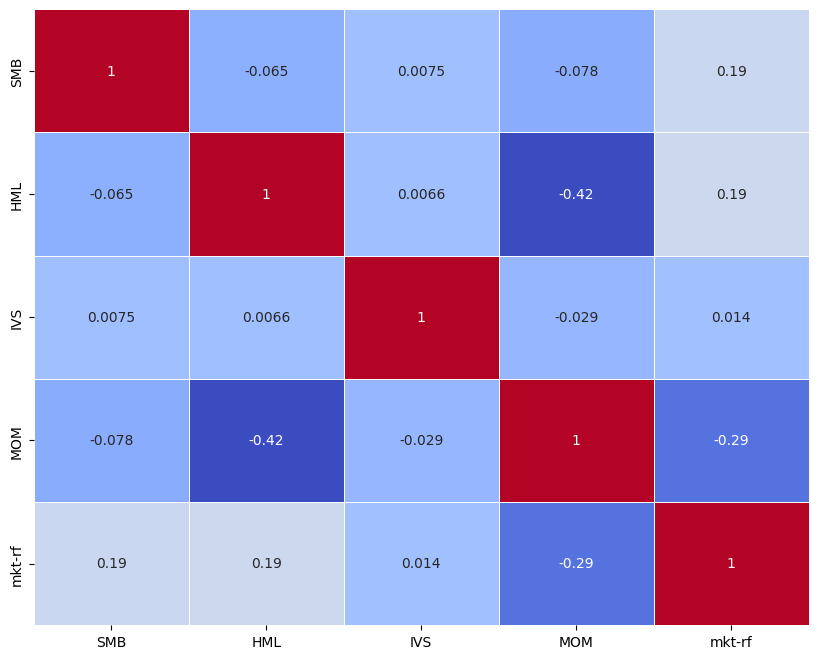
\includegraphics[width=300px]{assets/factors-corr-matrix.png}
    \caption{Correlation matrix for the five factors of the primary regression}
    \label{fig:factors-corr-matrix}
\end{figure}

\autoref{table:primary-regression-results} shows the results of the estimation of parameters for the cross section regression relative to equation \eqref{e:primary-regression}. In this regression, the whole time period of returns previously analyzed has been considered. Additionally, entity effects have been incorporated in the regression as they can serve to capture company specific information not captured by the rest of the factors as per \cite{ian_wagner_2019}. 

This main regression has been compared with other reference regressions. These follow the $CAPM$, Fama-French 3 factor model and the Carhart 4 factor model. This comparison has been performed in order to ensure the results given by the main regression are not spurious and fall in line with what more simple methods estimate for each of the drivers. Through the comparison of all regressions, a more robust result can be presented regarding the loadings for each of the factors. 

In \autoref{table:primary-regression-results} the t-statistic has also been included in parentheses below each estimated coefficient. No reference to the p-value of the t-statistic has been given as all coefficients are relevant at the $1\%$ level for all models. The $R^2$ has also been included. It can be noted how the $R^2$ increases with the number of factors as expected. The most significant jump is given by adding the two additional factors in the Fama-French model, with very little additional variance being explained by the $MOM$ and $IEP$ factors. The final model's $R^2$ stays at a moderate $2.67\%$, hinting at the idea that there may be other drivers at play needed to fully explain the performance of the strategy, hence why the secondary regression has been applied. Note that the number of observations in the regression is of 1.451.108 observations related to 398 different entities -- the 398 stocks remaining in the S\&P500 during the studied period. The F-statistic of the whole regression for the five factor model is 8004.8, demonstrating a joint significance for the model in addition to the individual significance of each of the coefficients. 

\begin{table}[ht]
    \centering
    \begin{tabular}{rcccc}
        \toprule
        Model & CAPM & FF3 & Carhart & Carhart+IEP \\ 
        \midrule
        $\alpha$ & 0.0005 & 0.0005 & 0.0005 & 0.0004 \\
                 & (98.5) & (99.0) & (98.9) & (63.3) \\[8px]
        $\beta_{mkt-rf}$ & -0.0560 & -0.0607 & -0.0631 & -0.0631 \\
                         & (-158.71) & (-166.1) & (-168.5) & (-168.5) \\[8px]
        $\beta_{SMB}$ & & 0.0783 & 0.0767 & 0.0766 \\
                      & & (106.6) & (104.2) & (104.1) \\[8px]
        $\beta_{HML}$ & & -0.0181 & -0.0249 & -0.0249 \\
                      & & (-33.7) & (-42.5) & (-42.5) \\[8px]
        $\beta_{MOM}$ & & & -0.0137 & -0.0135 \\
                      & & & (-29.4) & (-28.9) \\[8px]
        $\gamma$ & & & & 0.1085 \\
                       & & & & (9.4) \\[8px]
        \midrule
        $R^2$ & 1.71\% & 2.61\% & 2.66\% & 2.67\% \\

        \bottomrule
    \end{tabular}
    \caption{Coefficient estimations for the primary factor regression}
    \label{table:primary-regression-results}
\end{table}

Several observations can be made from the results of the coefficient estimations of the different models. The first of them is the robustness of the estimations. For all of the models, the coefficient estimations are pretty much the same for the different factor loadings. This showcases the orthogonality of the different factors, already hinted at by the low correlation shown in \autoref{fig:factors-corr-matrix}. It also indicates how there very likely is no omitted variable bias where the missing variable was being explained by one or more of the present factors and the models are correctly specified.

Regarding the coefficients themselves, it can be seen how, as already shown in the section \nameref{sec:overall-performance}, the strategy has a negative correlation to the market. It can also be seen how the strategy has a positive relation to the size factor and negative to the momentum and value factors. The negative exposure to the momentum could be expected, given how this strategy is in its essence a mean reverting strategy. However, it is interesting to see how the outperformance of low value and low size companies are key drivers of the performance of the strategy. 

Finally, regarding the Idiosyncratic Equity Volatility Premium, it can be seen how the strategy has a great exposure to this factor. Its performance seems to be greatly driven by high exposure to stocks with high idiosyncratic volatility premium, which again is to be expected as higher volatility leads to more opportunities to enter a position away from the long term equilibrium and thus more opportunities to profit when the stocks return to their cointegration equilibrium. More specifically, an increase in 1\% for the Idiosyncratic Equity Volatility Premium across stocks leads to an increase of 0.1 percentage point in the daily returns of the strategy. These companies can be found in sectors with rapid innovation, frequent regulatory changes or high sensitivity to firm-specific news, like the technology sector, or the pharmacetical or biotechnology sectors, with companies such as Tesla, Nvidia or Moderna being examples of specific stocks. 

Finally, there seems to be a consistent $\alpha$ of unexplained performance by the used five factor model. This $\alpha$ of 0.04\% in daily returns is a very significant 10.08\% in annual outperformance over the five factor benchmark model. 

\subsubsection{Secondary regression}
As it could be seen in the previous section, the five factor model used to understand the drivers of the strategy was very robust and it pointed the light at some of the key drivers of the strategy's performance. However, the low $R^2$ hints at the possibility of uncovering more of its drivers through more variables. 

In order to achieve that, the previous regression is performed on a rolling basis with quarterly data and a cross section regression is performed with company data on the different $\alpha$ obtained on those regressions. 

But first, a preliminary look at the correlation between the different factors can be useful to understand what information these may share among themselves. 

\begin{figure}[ht]
    \centering
    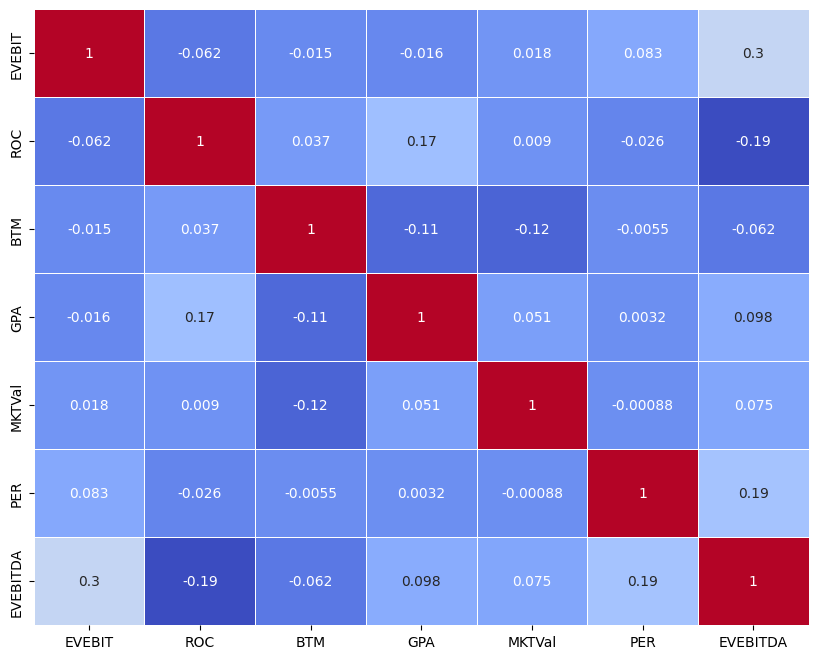
\includegraphics[width=300px]{assets/factors-secondary-corr-matrix.png}
    \caption{Correlation matrix for the seven factors of the secondary regression}
    \label{fig:factors-secondary-corr-matrix}
\end{figure}

The first thing to note in \autoref{fig:factors-secondary-corr-matrix} is the low correlation among the seven different factors, with the highest being a correlation of 30\%. This highest value is unsurprisingly that between $EVEEBIT$ and $EVEBITDA$, variables which transmit similar value related information, but which however are not as similar as the names may suggest. The next highest values are between $ROC$ and $GPA$, both profitability related metrics, and between $ROC$ and $EVEBITDA$, but even these third and seconds highest correlation pairs have a correlation of below 20\%. Most of the values are in the single digits, sign of the high orthogonality between most pairs of assets. 

The first secondary regression, with all factors indicated in the model shown in equation \eqref{eq:secondary-regression} and already presented in \autoref{fig:factors-secondary-corr-matrix}, has had the coefficients estimated on the alphas of all available quarters with the information of all available companies. The results of the estimation can be found in \autoref{table:secondary-regression-results-1}.

In this regression the $R^2$ achieved is of 1.09\%. There are 58 consecutive time periods corresponding for the 58 consecutive quarters in the studied period. The regression is jointly significant at all significance values with an F-statistic of 32.6. Again, individual entity effects are included as per \cite{ian_wagner_2019}. 
\begin{table}[ht]
    \centering
    \begin{tabular}{rccc}
        \toprule
        Coefficient & Estimation & t-statistic & p-value \\ 
        \midrule
        $\alpha$ & -0.0011 & -5.8 & 0.0000 \\
        $\gamma_{MKTVal}$ & 0.014 & 8.2 & 0.0000 \\
        $\gamma_{GPA}$ & 8.3e-5 & 0.8 & 0.3989 \\
        $\gamma_{ROC}$ & 0.0008 & 2.0 & 0.0443 \\
        $\gamma_{EVEBIT}$ & -0.0002 & -0.4 & 0.6612 \\
        $\gamma_{EVEBITDA}$ & 0.0007 & 4.1 & 0.0000 \\
        $\gamma_{PER}$ & 0.0005 & 0.8 & 0.4448 \\
        $\gamma_{BTM}$ & -0.0046 & -10.0 & 0.0000 \\
        \bottomrule
    \end{tabular}
    \caption{Coefficient estimations for the secondary factor regression}
    \label{table:secondary-regression-results-1}
\end{table}

However, even though the regression is jointly significant there are some coefficients which are not. Given the low shared information between the different factors, this is probably due to the outperformance of the strategy being unrelated to the information provided by some of these metrics. 

Through a process of iterative elimination of non significant variables, a final regression with more significant paramteters is obtained. 

\begin{table}[ht]
    \centering
    \begin{tabular}{rccc}
        \toprule
        Coefficient & Estimation & t-statistic & p-value \\ 
        \midrule
        $\alpha$ & -0.0011 & -5.9 & 0.0000 \\
        $\gamma_{MKTVal}$ & 0.014 & 8.2 & 0.0000 \\
        $\gamma_{ROC}$ & 0.0009 & 2.3 & 0.0192 \\
        $\gamma_{EVEBITDA}$ & 0.0007 & 4.1 & 0.0000 \\
        $\gamma_{BTM}$ & -0.0047 & -10.1 & 0.0000 \\
        \bottomrule
    \end{tabular}
    \captionsetup{justification=centering}
    \caption{Coefficient estimations for the secondary factor regression after iterative variable elimination}
    \label{table:secondary-regression-results-2}
\end{table}

In this final regression, all parameters are significant at all significance level, except for the Return on Capital which is singificant at the 5\% confidence level. 

The first interesting piece of information, like with Sherlock's dog, is given by what is missing. All factors that have been dropped due to their low significance -- namely Gross Profit over Assets, Enterprise Value to EBIT and Price to Earnings ratio -- can be inferred not to be drivers of the performance of the strategy. That is, those measures seem to be irrelevant to how the strategy performs, so including or removing assets based on those factors alone shouldn't have any significant impact given all other factors remain unchanged. 

According to \autoref{table:secondary-regression-results-2}, the strategy seems to outperform due to the assets with high market capitalization in the most significant way, but also due to those on the higher end of the valuation spectrum according to the $BTM$, same according to the $EVEBITDA$ and  with high profitability according to $ROC$. Note however how this could be due to sectoral preferences. The tech sector for example fits the description for all factors, so it could also be that the overperformance of the strategy is accentuated due to exposure to this sector wich has historically outperformed. This showcases the difference in the investment selection between this strategy and traditional rules-based strategies. These strategies which use fundamental factors generally tend to leave out investments in the technology sector due to having some undesirable ratios (e.g. PE ratio above the investment criteria threshold). This strategy thus lacks this bias which has burdened the performance of many such traditional strategies.